\documentclass[11pt,a4paper]{article}
\usepackage[T1]{fontenc}
\usepackage[utf8]{inputenc}
\usepackage{lmodern}
\usepackage{textcomp}
\usepackage[left=1.8cm,right=1.8cm,top=3.0cm,bottom=2.2cm,headheight=36pt,headsep=12pt]{geometry}
\usepackage{multicol}
\usepackage{xcolor}
\usepackage{fancyhdr}\usepackage{tikz}
\usepackage{graphicx}
\usepackage{array}
\usepackage{amsmath,amssymb}
\usepackage{setspace}
\usepackage{longtable}
\graphicspath{{../}}
\definecolor{ygreen}{RGB}{46,139,87}\definecolor{dgreen}{RGB}{28,90,56}
\renewcommand{\normalsize}{\fontsize{10.9}{13.4}\selectfont}
\renewcommand{\familydefault}{\rmdefault}
\setlength{\parindent}{0pt}
\setlength{\columnsep}{0.8cm}
\setlength{\columnseprule}{0.4pt}
\setlength{\multicolsep}{3pt plus 1pt minus 1pt}
\renewcommand{\textsubscript}[1]{\ensuremath{_{\text{\fontsize{8}{8}\selectfont #1}}}}
\renewcommand{\textsuperscript}[1]{\ensuremath{^{\text{\fontsize{8}{8}\selectfont #1}}}}
\newcommand{\qn}[1]{\textbf{\fontsize{11.5}{13}\selectfont #1}}
\newcommand{\qsep}{\par\vspace{13pt}}
\newcommand{\fwrule}{\par\vspace{5pt}\noindent\rule{\linewidth}{1.4pt}\par\vspace{7pt}}
\newsavebox{\fitb}
\newcommand{\fitbox}[1]{\sbox{\fitb}{#1}\ifdim\wd\fitb>\linewidth\resizebox{\linewidth}{!}{\usebox{\fitb}}\else\usebox{\fitb}\fi}
\newcommand{\diqqat}[1]{\par\smallskip\noindent\textbf{Diqqat!} #1\par\medskip}
\newcommand{\javob}{\par\nopagebreak[4]\smallskip\noindent\textbf{Javob:} \rule[-2pt]{7.5cm}{0.4pt}\par\smallskip\noindent\textbf{Diqqat!} Javobingizni javoblar varaqasiga ko`chirib yozing.\par\medskip}
\pagestyle{fancy}
\fancyhf{}
\renewcommand{\headrulewidth}{1.6pt}\renewcommand{\headrule}{{\color{ygreen}\hrule height 1.6pt width\headwidth}}
\newcommand{\hdrlogo}{
\begin{tikzpicture}[baseline=0pt]\fill[ygreen,rounded corners=3pt] (0,0) rectangle (0.95,0.95);\node[white,font=\fontsize{24}{26}\bfseries\selectfont] at (0.475,0.47){K};\node[anchor=west,font=\fontsize{16}{18}\bfseries\selectfont,text=dgreen] at (1.15,0.66){KIMYO};\node[anchor=west,font=\footnotesize\scshape,text=gray] at (1.15,0.2){Milliy sertifikat\ \ 2026};\end{tikzpicture}}
\newcommand{\hdrpill}[1]{\begin{tikzpicture}[baseline=0pt]\node[fill=ygreen,text=white,rounded corners=8pt,inner xsep=10pt,inner ysep=5pt,font=\fontsize{13}{15}\bfseries\selectfont] at (0,0.475){#1};\end{tikzpicture}}
\fancyhead[L]{\hdrlogo}
\fancyhead[R]{\hdrpill{10-variant}}

\fancyfoot[C]{\thepage}
\fancypagestyle{first}{\fancyhf{}\renewcommand{\headrulewidth}{1.6pt}\renewcommand{\headrule}{{\color{ygreen}\hrule height 1.6pt width\headwidth}}\fancyhead[L]{\hdrlogo}\fancyhead[R]{\hdrpill{10-variant}}\fancyfoot[C]{\thepage}}
\begin{document}
\normalsize
\thispagestyle{first}
\noindent\textit{Davriy jadvaldan foydalanish mumkin.}
\par\smallskip
\begin{multicols}{2}
\noindent\qn{1.} PCl\textsubscript{5} $\rightleftarrows$ PCl\textsubscript{3} + Cl\textsubscript{2} reaksiyasi 1 l hajmli idishda o`tkazildi. Ma'lumotlar jadvalda berilgan:
\begin{center}
\renewcommand{\arraystretch}{1.15}
\fitbox{\begin{tabular}{|c|c|c|}\hline
\textbf{Modda} & \textbf{PCl\textsubscript{5}} & \textbf{PCl\textsubscript{3}} \\ \hline
Boshlang`ich, mol & 6 & 0 \\ \hline
Muvozanatda, mol & --- & 0,5 \\ \hline
\end{tabular}}
\end{center}
Muvozanat \textbf{konstantasini (K) hisoblang.}

\noindent A)~\textsl{0,091} \hfill B)~\textsl{0,045} \hfill C)~\textsl{0,023} \hfill D)~\textsl{22}\par
\qsep
\noindent\qn{2.} 10 l SO\textsubscript{2} va 10 l O\textsubscript{2} aralashmasi reaksiyaga kirishdi (2SO\textsubscript{2} + O\textsubscript{2} $\to$ 2SO\textsubscript{3}, hamma moddalar bir xil sharoitda gaz holida). Reaksiyadan keyingi gaz aralashmasining \textbf{hajmini (l) aniqlang.}

\noindent A)~\textsl{15} \hfill B)~\textsl{20} \hfill C)~\textsl{10} \hfill D)~\textsl{5}\par
\qsep
\noindent\qn{3.} KClO\textsubscript{3} tarkibida Cl ning oksidlanish \textbf{darajasini aniqlang.}

\noindent A)~\textsl{+6} \hfill B)~\textsl{+7} \hfill C)~\textsl{+5} \hfill D)~\textsl{$-$2}\par
\qsep
\noindent\qn{4.} Azot atomining p- va d- pog`onachalaridagi elektronlardan nechtasining magnit kvant soni m\_l = 1 ga teng? (\textit{Z} = 7)

\noindent A)~\textsl{2} \hfill B)~\textsl{1} \hfill C)~\textsl{4} \hfill D)~\textsl{3}\par
\qsep
\noindent\qn{5.} 1 mol AlCl\textsubscript{3} va 3 mol Ba(OH)\textsubscript{2} suvda eritilib, eritma hajmi 2 l ga yetkazildi. Eritmadagi barcha ionlarning umumiy molyar \textbf{konsentratsiyasini (mol/l) aniqlang} (kuchli elektrolitlar to`liq dissotsilanadi).

\noindent A)~\textsl{2} \hfill B)~\textsl{13} \hfill C)~\textsl{3,25} \hfill D)~\textsl{6,5}\par
\qsep
\noindent\qn{6.} 16,8 g CaO va 8,1 g H\textsubscript{2}O aralashtirilib, reaksiya o`tkazildi (CaO + H\textsubscript{2}O $\to$ Ca(OH)\textsubscript{2}). Hosil bo`lgan Ca(OH)\textsubscript{2} \textbf{massasini (g) aniqlang.}

\noindent A)~\textsl{33,3} \hfill B)~\textsl{44,4} \hfill C)~\textsl{22,2} \hfill D)~\textsl{11,1}\par
\qsep
\noindent\qn{7.} N\textsubscript{2} + 3H\textsubscript{2} $\rightleftarrows$ 2NH\textsubscript{3} reaksiyada muvozanat qaror topganda [N\textsubscript{2}] = 1, [H\textsubscript{2}] = 1, [NH\textsubscript{3}] = 4 mol/l bo`ldi. N\textsubscript{2} ning boshlang`ich \textbf{konsentratsiyasini (mol/l) aniqlang.}

\noindent A)~\textsl{3} \hfill B)~\textsl{1} \hfill C)~\textsl{5} \hfill D)~\textsl{6}\par
\qsep
\noindent\qn{8.} Gazlar aralashmasi tarkibi jadvalda berilgan (n.sh.):
\begin{center}
\renewcommand{\arraystretch}{1.15}
\fitbox{\begin{tabular}{|c|c|}\hline
\textbf{Gaz} & \textbf{Hajmi, l} \\ \hline
NH\textsubscript{3} & 1 \\ \hline
SO\textsubscript{2} & 3 \\ \hline
O\textsubscript{2} & 3 \\ \hline
\end{tabular}}
\end{center}
Aralashmaning havoga nisbatan \textbf{zichligini aniqlang} (M(havo) = 29 g/mol).

\noindent A)~\textsl{3} \hfill B)~\textsl{1,5} \hfill C)~\textsl{0,75} \hfill D)~\textsl{43,57}\par
\qsep
\noindent\qn{9.} 300 g 10\% li Na\textsubscript{2}SO\textsubscript{4} eritmasiga 25 g shu tuzning o`zi qo`shilib eritildi. Hosil bo`lgan eritmaning massa \textbf{ulushini (\%) aniqlang.}

\noindent A)~\textsl{16,92} \hfill B)~\textsl{18,33} \hfill C)~\textsl{9,17} \hfill D)~\textsl{13,54}\par
\qsep
\noindent\qn{10.} Azot (\textit{Z} = 7) atomining tashqi energetik pog`onasidagi elektronlar \textbf{sonini aniqlang.}

\noindent A)~\textsl{6} \hfill B)~\textsl{4} \hfill C)~\textsl{5} \hfill D)~\textsl{7}\par
\qsep
\noindent\qn{11.} Quyidagi zarrachalardan qaysilari argon atomi bilan izoelektron? 1) Na\textsuperscript{+}; 2) Cl\textsuperscript{$-$}; 3) Ca\textsuperscript{2+}; 4) K\textsuperscript{+}

\noindent A)~\textsl{2, 4} \hfill B)~\textsl{1, 3, 4} \hfill C)~\textsl{2, 3, 4} \hfill D)~\textsl{1, 4}\par
\qsep
\noindent\qn{12.} KNO\textsubscript{3} va NaCl eruvchanligining haroratga bog`liqligi grafikda berilgan.
\begin{center}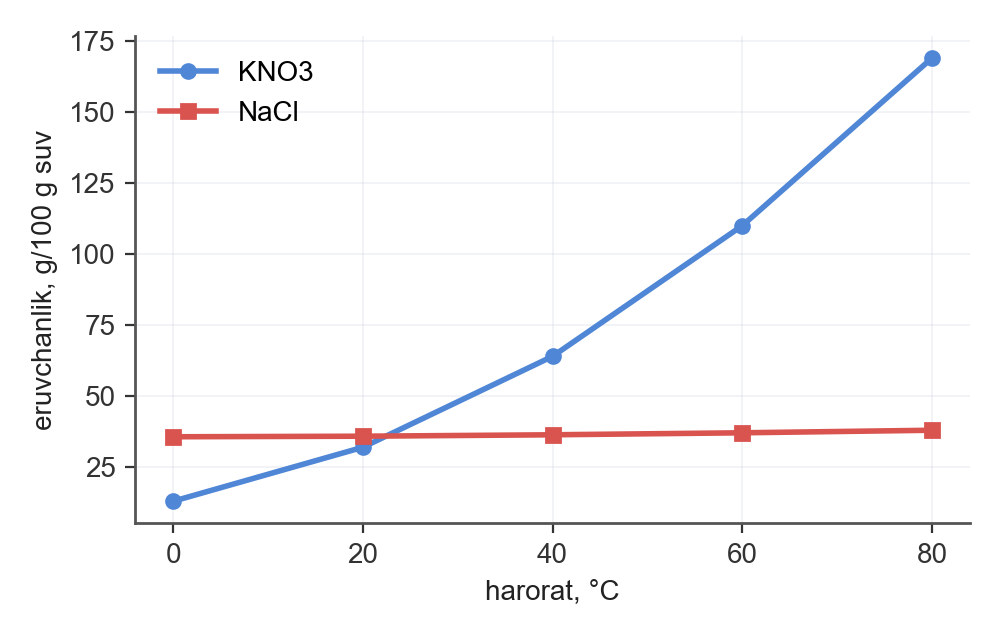
\includegraphics[width=0.86\linewidth]{rasmlar/gen/s2_v10_0.png}\end{center}
60 \textdegree{}C da qaysi tuzning eruvchanligi katta?

\noindent A)~\textsl{NaCl} \hfill B)~\textsl{KCl} \hfill C)~\textsl{NH\textsubscript{4}Cl} \hfill D)~\textsl{KNO\textsubscript{3}}\par
\qsep
\noindent\qn{13.} 16,1 g Na\textsubscript{2}SO\textsubscript{4}$\cdot$10H\textsubscript{2}O 100 g suvda eritildi. Eritmadagi tuzning massa \textbf{ulushini (\%) aniqlang.}

\noindent A)~\textsl{7,1} \hfill B)~\textsl{13,87} \hfill C)~\textsl{12,23} \hfill D)~\textsl{6,12}\par
\qsep
\noindent\qn{14.} Quyidagi tuzlardan qaysilari asosli tuz? 1) K\textsubscript{2}SO\textsubscript{4}; 2) (CuOH)\textsubscript{2}CO\textsubscript{3}; 3) CaCO\textsubscript{3}; 4) KAl(SO\textsubscript{4})\textsubscript{2}

\noindent A)~\textsl{2, 4} \hfill B)~\textsl{2} \hfill C)~\textsl{2, 3} \hfill D)~\textsl{4}\par
\qsep
\noindent\qn{15.} CaCO\textsubscript{3} $\to$ CaO + CO\textsubscript{2} jarayoni uchun 50 g CaCO\textsubscript{3} olingan (unum 90\%). CaO \textbf{massasini (g) aniqlang.}

\noindent A)~\textsl{28} \hfill B)~\textsl{50,4} \hfill C)~\textsl{25,2} \hfill D)~\textsl{12,6}\par
\qsep
\noindent\qn{16.} Nodir gazlar haqida qaysi fikrlar to`g`ri? 1) Argon elektr lampalarida ishlatiladi; 2) Nodir gazlar odatiy sharoitda ko`p atomli molekulalar hosil qiladi; 3) Nodir gazlar kimyoviy jihatdan juda faol; 4) Neon reklama naylarida ishlatiladi

\noindent A)~\textsl{1, 2, 3} \hfill B)~\textsl{2, 3} \hfill C)~\textsl{3, 4} \hfill D)~\textsl{1, 4}\par
\qsep
\noindent\qn{17.} 2NaNO\textsubscript{3} $\to$ 2NaNO\textsubscript{2} + O\textsubscript{2} reaksiyasida tarkibida 60\% aralashma bo`lgan 42,5 g namuna (asosiy modda NaNO\textsubscript{3}) ishtirok etdi. NaNO\textsubscript{2} \textbf{massasini (g) toping.}

\noindent A)~\textsl{27,6} \hfill B)~\textsl{6,9} \hfill C)~\textsl{13,8} \hfill D)~\textsl{20,7}\par
\qsep
\noindent\qn{18.} 60 g FeS\textsubscript{2} yondirilib, hosil bo`lgan SO\textsubscript{2} dan H\textsubscript{2}SO\textsubscript{4} olindi (jami unum 100\%). Sulfat kislota \textbf{massasini (g) aniqlang.}

\noindent A)~\textsl{98} \hfill B)~\textsl{49} \hfill C)~\textsl{196} \hfill D)~\textsl{147}\par
\qsep
\noindent\qn{19.} KNO\textsubscript{3} qizdirilganda qanday moddalar hosil bo`ladi?

\noindent\begin{tabular}{@{}p{0.47\linewidth}@{}p{0.47\linewidth}@{}}
A)~\textsl{N\textsubscript{2}O va H\textsubscript{2}O} & B)~\textsl{Ag, NO\textsubscript{2} va O\textsubscript{2}} \\
C)~\textsl{KNO\textsubscript{2} va O\textsubscript{2}} & D)~\textsl{CuO, NO\textsubscript{2} va O\textsubscript{2}} \\
\end{tabular}\par
\qsep
\noindent\qn{20.} Rasmda uchta uglevodorodning tuzilish formulasi berilgan.
\begin{center}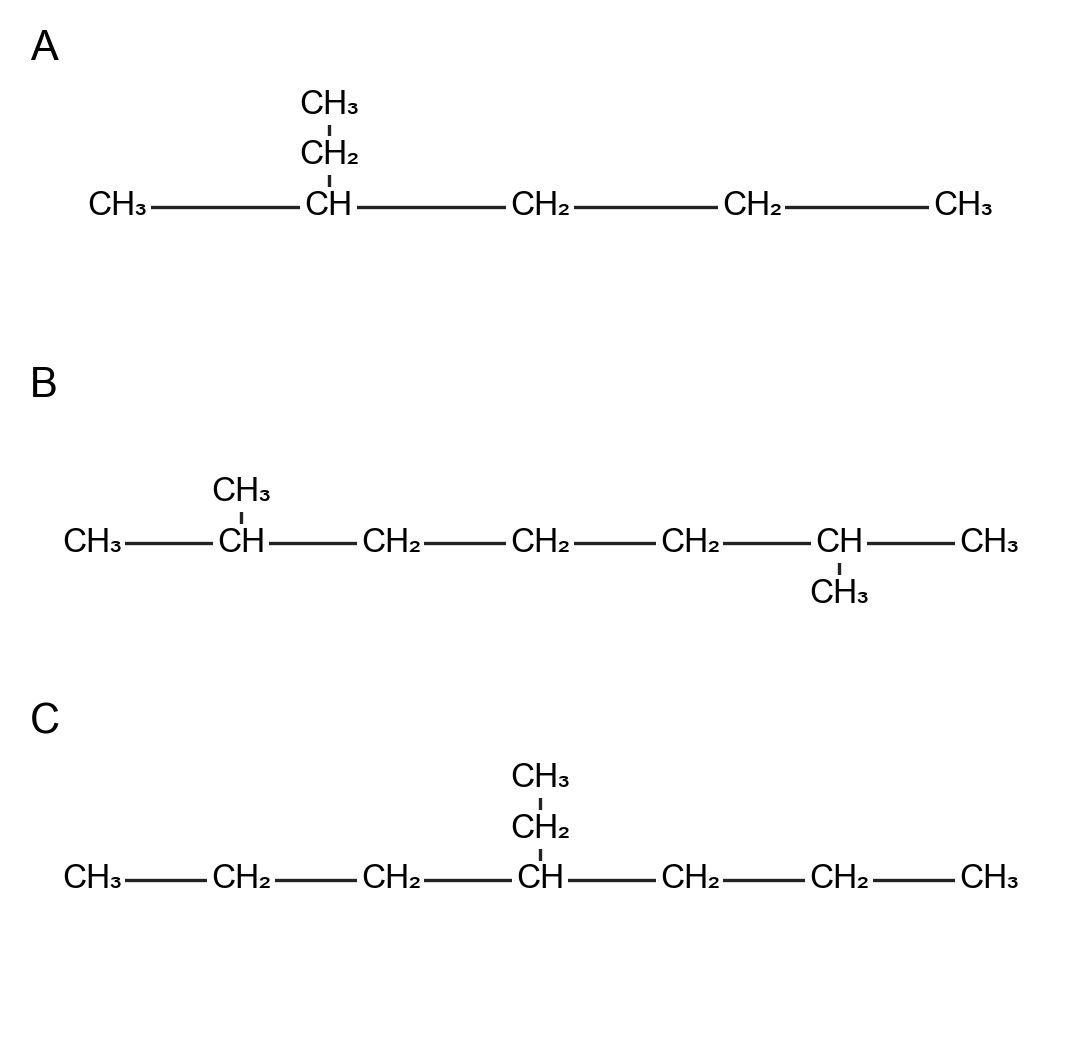
\includegraphics[width=0.86\linewidth]{rasmlar/gen/is_479186.png}\end{center}
Qaysi juftlik o`zaro izomerlar hisoblanadi?

\noindent A)~\textsl{A va B} \hfill B)~\textsl{A va C} \hfill C)~\textsl{A, B va C} \hfill D)~\textsl{B va C}\par
\qsep
\noindent\qn{21.} CH\textsubscript{2}=CH--CH\textsubscript{2}--CH\textsubscript{3} birikmaning sistematik nomi qaysi qatorda to`g`ri keltirilgan?

\noindent A)~\textsl{buten-2} \hfill B)~\textsl{buten-1} \hfill C)~\textsl{1-butin} \hfill D)~\textsl{butan}\par
\qsep
\noindent\qn{22.} Arenlar, neft va tabiiy gaz haqida qaysi fikrlar to`g`ri? 1) Benzol bromli suvni rangsizlantirmaydi; 2) Tabiiy gazning asosiy qismi propan; 3) Neft fraksiyalaridan gazolin 150 \textdegree{}C gacha haydaladi; 4) Benzoldan nitrobenzol nitrolash bilan olinadi

\noindent A)~\textsl{3, 4} \hfill B)~\textsl{1, 2} \hfill C)~\textsl{1, 3, 4} \hfill D)~\textsl{2, 3, 4}\par
\qsep
\noindent\qn{23.} C\textsubscript{2}H\textsubscript{5}OH + CuO (t) reaksiyasi natijasida qaysi organik modda hosil bo`ladi?

\noindent\begin{tabular}{@{}p{0.47\linewidth}@{}p{0.47\linewidth}@{}}
A)~\textsl{sirka aldegid} & B)~\textsl{etilen} \\
C)~\textsl{etanol} & D)~\textsl{asetilen} \\
\end{tabular}\par
\qsep
\noindent\qn{24.} Aldegid va ketonlar haqida qaysi fikrlar to`g`ri? 1) Formalin --- formaldegidning 40\% li eritmasi; 2) Aldegidlar qaytarilganda ikkilamchi spirt hosil bo`ladi; 3) Sirka aldegid Kucherov reaksiyasi bilan olinadi; 4) Ketonlar kuchsiz oksidlovchilar bilan oksidlanmaydi

\noindent A)~\textsl{2, 3, 4} \hfill B)~\textsl{1, 3} \hfill C)~\textsl{1, 4} \hfill D)~\textsl{1, 3, 4}\par
\qsep
\noindent\qn{25.} CH\textsubscript{3}COOH + C\textsubscript{2}H\textsubscript{5}OH $\to$ CH\textsubscript{3}COOC\textsubscript{2}H\textsubscript{5} + H\textsubscript{2}O jarayoni uchun 46 g C\textsubscript{2}H\textsubscript{5}OH olingan (unum 75\%). CH\textsubscript{3}COOC\textsubscript{2}H\textsubscript{5} \textbf{massasini (g) aniqlang.}

\noindent A)~\textsl{88} \hfill B)~\textsl{132} \hfill C)~\textsl{33} \hfill D)~\textsl{66}\par
\qsep
\noindent\qn{26.} Murakkab efirlar va yog`lar haqida qaysi fikrlar to`g`ri? 1) Murakkab efirlarning gidrolizi ishqoriy muhitda qaytmas; 2) Suyuq yog`larni gidrogenlab qattiq yog` olinadi; 3) Sovun --- yuqori yog` kislotalarning natriyli tuzi; 4) Suyuq yog`lar to`yinmagan kislotalardan hosil bo`lgan

\noindent\begin{tabular}{@{}p{0.47\linewidth}@{}p{0.47\linewidth}@{}}
A)~\textsl{1, 2, 3, 4} & B)~\textsl{1, 2, 3} \\
C)~\textsl{1, 3, 4} & D)~\textsl{1, 2, 4} \\
\end{tabular}\par
\qsep
\noindent\qn{27.} 68,4 g saxaroza gidrolizlanganda necha gramm glyukoza hosil bo`ladi?

\noindent A)~\textsl{36} \hfill B)~\textsl{68,4} \hfill C)~\textsl{72} \hfill D)~\textsl{18}\par
\qsep
\noindent\qn{28.} 26,7 g alanin HCl bilan reaksiyaga kirishganda hosil bo`lgan tuz \textbf{massasini (g) aniqlang.}

\noindent A)~\textsl{26,7} \hfill B)~\textsl{10,95} \hfill C)~\textsl{75,3} \hfill D)~\textsl{37,65}\par
\qsep
\noindent\qn{29.} C\textsubscript{2}H\textsubscript{4} + Cl\textsubscript{2} $\to$ C\textsubscript{2}H\textsubscript{4}Cl\textsubscript{2} reaksiyasida 4,48 l (n.sh.) Cl\textsubscript{2} ishtirok etdi. C\textsubscript{2}H\textsubscript{4}Cl\textsubscript{2} \textbf{massasini (g) toping.}

\noindent A)~\textsl{39,6} \hfill B)~\textsl{19,8} \hfill C)~\textsl{9,9} \hfill D)~\textsl{29,7}\par
\qsep
\noindent\qn{30.} Rasmdagi asbobda 6,5 g rux mo`l xlorid kislota bilan reaksiyaga kirishdi (Zn + 2HCl $\to$ ZnCl\textsubscript{2} + H\textsubscript{2}). Ajralgan vodorodning \textbf{hajmini (l, n.sh.) aniqlang.}
\begin{center}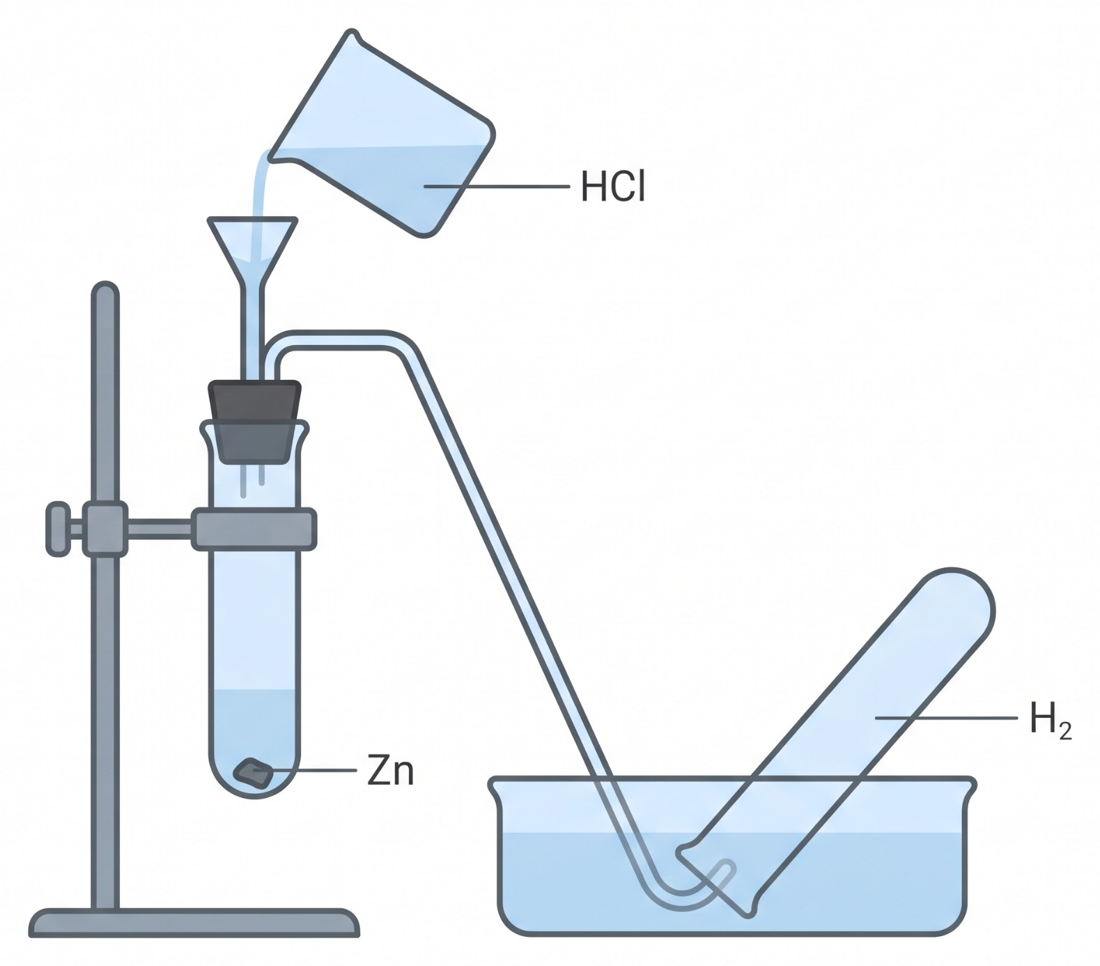
\includegraphics[width=0.86\linewidth]{rasmlar/darslik/d_vodorod.png}\end{center}

\noindent A)~\textsl{4,48} \hfill B)~\textsl{2,24} \hfill C)~\textsl{1,12} \hfill D)~\textsl{0,1}\par
\qsep
\noindent\qn{31.} 200 g 30\% li va 100 g 50\% li Na\textsubscript{2}SO\textsubscript{4} eritmalari aralashtirildi. Yangi eritmaning massa \textbf{ulushini (\%) toping.}

\noindent A)~\textsl{36,67} \hfill B)~\textsl{40} \hfill C)~\textsl{80} \hfill D)~\textsl{33}\par
\qsep
\noindent\qn{32.} Kimyoviy laboratoriyada o`lchov silindri nima uchun ishlatiladi?
\noindent A)~\textsl{eritmaning kichik hajmlarini o`lchab olish}\par
\noindent B)~\textsl{suyuqlik hajmini o`lchash}\par
\noindent C)~\textsl{eritmalarni bug`latish}\par
\noindent D)~\textsl{titrlashda reagent hajmini aniq o`lchash   ---}\par
\qsep
\end{multicols}
\medskip
\noindent\setlength{\fboxsep}{0pt}\fbox{\begin{tabular}{p{0.74\linewidth}|p{0.2\linewidth}}
\parbox[t]{0.72\linewidth}{\vspace{3pt}\textbf{Topshiriqlar (33--35) va javob variant (A--F)larini o`zaro to`g`ri moslashtiring.} Etanol va fenoldan iborat 28 g aralashma natriy bilan to`liq reaksiyaga kirishganda 4,48 l (n.sh.) vodorod ajraldi. Xuddi shu massadagi aralashma NaOH eritmasi bilan (faqat fenol) va bromli suv bilan (faqat fenol) ham reaksiyaga kirishadi.
\vspace{3pt}} & \parbox[t]{0.19\linewidth}{\vspace{3pt}A~\textsl{67,14}\\[3pt]
B~\textsl{47,66}\\[3pt]
C~\textsl{8}\\[3pt]
D~\textsl{119,16}\\[3pt]
E~\textsl{59,58}\\[3pt]
F~\textsl{12}}\\ \hline
\parbox[t]{0.72\linewidth}{\vspace{2pt}\textbf{33. Aralashmadagi fenol massa ulushini (\%) aniqlang.}\vspace{2pt}} & \\ \hline
\parbox[t]{0.72\linewidth}{\vspace{2pt}\textbf{34. Fenolni to`liq neytrallash uchun zarur NaOH massasini (g) aniqlang.}\vspace{2pt}} & \\ \hline
\parbox[t]{0.72\linewidth}{\vspace{2pt}\textbf{35. Mo`l bromli suv bilan reaksiyada hosil bo`lgan tribromfenol massasini (g) aniqlang (reaksiya unumi 90\%).}\vspace{2pt}} & 
\end{tabular}}
\par\bigskip
\noindent\qn{36.} Cu + HNO\textsubscript{3} $\to$ Cu(NO\textsubscript{3})\textsubscript{2} + NO\textsubscript{2} + H\textsubscript{2}O reaksiya tenglamasini tenglang va barcha koeffitsiyentlar \textbf{yig`indisini aniqlang.}
\javob\qsep
\noindent\qn{37.} Ketma-ket ulangan ikkita elektrolizyordan (CuSO\textsubscript{4} va AgNO\textsubscript{3} eritmalari, inert elektrodlar) tok o`tkazildi. Birinchi elektrolizyor katodida 12,8 g mis ajraldi. Ikkala elektrolizyor anodlarida ajralgan kislorodning umumiy \textbf{hajmini (l, n.sh.) toping} (anodda ikkalasida ham O\textsubscript{2} ajraladi).
\javob\qsep
\noindent\qn{38.} Alyuminiy va kalsiy dan iborat 13,4 g aralashma mo`l xlorid kislotada eritilganda 11,2 l (n.sh.) vodorod ajraldi. Aralashmadagi alyuminiyning massa \textbf{ulushini (\%) aniqlang.}
\javob\qsep
\noindent\qn{39.} 61,5 g nitrobenzoldan anilin olishda unum 75\% bo`lsa, mahsulot \textbf{massasini (g) aniqlang.}
\javob\qsep
\noindent\qn{40.} 22,2 g propion kislota va 9,6 g metanol dan 75\% unum bilan murakkab efir olindi. Efir \textbf{massasini (g) toping.}
\javob\qsep
\par\bigskip\begin{center}\textbf{\fontsize{13}{15}\selectfont YOZMA ISH}\end{center}
\noindent\qn{41.} \textbf{Topshiriqni bajarish jarayonida barcha reaksiya tenglamalarini yozing. Miqdoriy va arifmetik hisoblashlarni (unga asos bo`lgan usul yoki formulani ko`rsatgan holda) uzviy ketma-ketlikda bajaring.}\par\smallskip
1,2 g noma'lum metall kislota bilan to`liq reaksiyaga kirishib, 1,12 l (n.sh.) vodorod ajratdi. (Vodorodning ekvivalent hajmi \textit{V}\_E(H\textsubscript{2}) = 11,2 l/mol.)\par
\noindent 1)\ Metallning ekvivalent massasini (g/mol) hisoblang.\par
\noindent 2)\ Metallning valentligi 2 bo`lsa, uning atom massasini hisoblab, metallni aniqlang. Ajralgan vodorodning massasini (g) ham hisoblang.\par
\noindent 3)\ Shu metallning oksidi formulasini yozing va molyar massasini hisoblang.\par
\noindent 4)\ 1,2 g metall to`liq yonganda hosil bo`lgan oksid massasini (g) toping. Metall oksidining ekvivalent massasini (g/mol) ham aniqlang.\par
\noindent 5)\ Yonishga sarflangan kislorod hajmini (l, n.sh.) aniqlang. Shuningdek metall xloridida (MCl\textsubscript{2}) metallning massa ulushini (\%) toping.\par
\diqqat{Mazkur topshiriq kengaytirilgan javobni talab etib, uning yechilish usuli va shu usul asosidagi barcha hisoblash amallari javoblar varaqasida aks etishi lozim.}\qsep
\noindent\qn{42.} Quyidagi o`zgarishlar zanjirida \textit{X}, \textit{Y}, \textit{Z} noma'lum organik moddalar:\par
\[\setlength{\fboxsep}{0pt}\text{C\textsubscript{12}H\textsubscript{22}O\textsubscript{11}}\xrightarrow{\text{H\textsubscript{2}O, H\textsuperscript{+}}}\text{\textit{X}}\xrightarrow{\text{bijg`ish}}\text{\textit{Y}}\xrightarrow{\text{Na}}\text{C\textsubscript{2}H\textsubscript{5}ONa}\]
\noindent 1)\ C\textsubscript{12}H\textsubscript{22}O\textsubscript{11} $\to$ \textit{X} : reaksiya tenglamasini yozing; hosil bo`lgan moddani nomlang.\par
\noindent 2)\ \textit{X} $\to$ \textit{Y} : reaksiya tenglamasini yozing; hosil bo`lgan moddani nomlang.\par
\noindent 3)\ \textit{Y} $\to$ C\textsubscript{2}H\textsubscript{5}ONa : reaksiya tenglamasini yozing; hosil bo`lgan moddani nomlang.\par
\diqqat{Mazkur topshiriq kengaytirilgan javobni talab etib, uning yechilish usuli va shu usul asosidagi barcha hisoblash amallari javoblar varaqasida aks etishi lozim.}\qsep
\noindent\qn{43.} \textbf{Topshiriqni bajarish jarayonida barcha reaksiya tenglamalarini yozing. Miqdoriy va arifmetik hisoblashlarni (unga asos bo`lgan usul yoki formulani ko`rsatgan holda) uzviy ketma-ketlikda bajaring.}\par\smallskip
NaBr va NaI dan iborat 32,8 g aralashma suvda eritilib, mo`l xlor o`tkazildi. Eritma bug`latilib, qoldiq quritilganda uning massasi 14,62 g bo`ldi.\par
\noindent 1)\ Reaksiya tenglamalarini yozing. Aralashmadagi NaBr va NaI massalarini (g) toping.\par
\noindent 2)\ Sarflangan xlor hajmini (l, n.sh.) hisoblang. Hosil bo`lgan NaCl miqdorini (mol) ham toping.\par
\noindent 3)\ Ajralgan brom va yodning massalarini (g) toping.\par
\noindent 4)\ Dastlabki aralashma eritmasiga mo`l AgNO\textsubscript{3} qo`shilganda hosil bo`ladigan cho`kmalar massasini (g) aniqlang.\par
\noindent 5)\ Ajralgan brom va yod aralashmasida bromning massa ulushini (\%) toping.\par
\diqqat{Mazkur topshiriq kengaytirilgan javobni talab etib, uning yechilish usuli va shu usul asosidagi barcha hisoblash amallari javoblar varaqasida aks etishi lozim.}\qsep
\newpage
\noindent\textbf{\fontsize{13}{15}\selectfont 10-variant}\hfill \textbf{Javoblar kaliti}\par\smallskip\hrule\smallskip
\textit{Faqat o`qituvchi uchun.}\par\medskip
\noindent\textbf{1--32-savollar}\par\smallskip
\noindent\begin{tabular}{|c|c|c|c|c|c|c|c|c|c|c|c|c|c|c|c|}\hline
\textbf{1} & \textbf{2} & \textbf{3} & \textbf{4} & \textbf{5} & \textbf{6} & \textbf{7} & \textbf{8} & \textbf{9} & \textbf{10} & \textbf{11} & \textbf{12} & \textbf{13} & \textbf{14} & \textbf{15} & \textbf{16}\\\hline
\textsl{B} & \textsl{A} & \textsl{C} & \textsl{B} & \textsl{D} & \textsl{C} & \textsl{A} & \textsl{B} & \textsl{A} & \textsl{C} & \textsl{C} & \textsl{D} & \textsl{D} & \textsl{B} & \textsl{C} & \textsl{D}\\\hline
\textbf{17} & \textbf{18} & \textbf{19} & \textbf{20} & \textbf{21} & \textbf{22} & \textbf{23} & \textbf{24} & \textbf{25} & \textbf{26} & \textbf{27} & \textbf{28} & \textbf{29} & \textbf{30} & \textbf{31} & \textbf{32}\\\hline
\textsl{C} & \textsl{A} & \textsl{C} & \textsl{D} & \textsl{B} & \textsl{C} & \textsl{A} & \textsl{D} & \textsl{D} & \textsl{A} & \textsl{A} & \textsl{D} & \textsl{B} & \textsl{B} & \textsl{A} & \textsl{B}\\\hline
\end{tabular}\par\medskip
\noindent\textbf{33--35-savollar}\par\smallskip
\noindent\begin{tabular}{|c|c|c|}\hline \textbf{No} & \textbf{Javob} & \textbf{Qiymat}\\\hline
33 & \textsl{A} & 67,14\\\hline
34 & \textsl{C} & 8\\\hline
35 & \textsl{E} & 59,58\\\hline
\end{tabular}\par\medskip
\noindent\textbf{36--40-savollar}\par\smallskip
\noindent\begin{tabular}{|c|c|}\hline \textbf{No} & \textbf{To`g`ri javob}\\\hline
36 & 10\\\hline
37 & 4,48\\\hline
38 & 40,3\\\hline
39 & 34,88\\\hline
40 & 19,8\\\hline
\end{tabular}\par\medskip
\noindent\textbf{41--43-topshiriqlar: javoblar}\par\smallskip
\noindent\textbf{41-topshiriq.}\par
\noindent 1) 12 g/mol\par
\noindent 2) Mg; 0,1 g\par
\noindent 3) MgO; 40 g/mol\par
\noindent 4) 2 g; 20 g/mol\par
\noindent 5) 0,56 l; 25,3\%\par
\noindent\textbf{42-topshiriq.}\par
\noindent 1) C\textsubscript{12}H\textsubscript{22}O\textsubscript{11} + H\textsubscript{2}O, H\textsuperscript{+} $\to$ C\textsubscript{6}H\textsubscript{12}O\textsubscript{6} (glyukoza)\par
\noindent 2) C\textsubscript{6}H\textsubscript{12}O\textsubscript{6} + bijg`ish $\to$ C\textsubscript{2}H\textsubscript{5}OH (etanol)\par
\noindent 3) C\textsubscript{2}H\textsubscript{5}OH + Na $\to$ C\textsubscript{2}H\textsubscript{5}ONa (natriy etilat)\par
\noindent\textbf{43-topshiriq.}\par
\noindent 1) 10,3 g; 22,5 g\par
\noindent 2) 2,8 l; 0,25 mol\par
\noindent 3) 8 g; 19,05 g\par
\noindent 4) 54,05 g\par
\noindent 5) 29,6\%\par
\par\bigskip\noindent\textbf{Mavzular taqsimoti}\par\smallskip
{\small\noindent\begin{longtable}{|c|p{7.2cm}|p{5.4cm}|c|}\hline \textbf{No} & \textbf{Mavzu} & \textbf{Tekshiriladigan ko`nikma} & \textbf{Ball}\\\hline
1 & Tirkashev VI bob (muvozanat, jadval) & Jadval tahlili & 1\\\hline
2 & 8-sinf (Gey-Lyussak, Avogadro) & Hisoblash va masala yechish & 1\\\hline
3 & 8-sinf; Tirkashev \textit{V} bob (oksidlanish darajasi) & Bilim va tushunish & 1\\\hline
4 & Tirkashev I bob (kvant sonlari) & Bilim va tushunish & 1\\\hline
5 & Tirkashev IV bob (kuchli elektrolitlar) & Hisoblash va masala yechish & 1\\\hline
6 & 8-sinf (ortiqcha modda masalasi) & Hisoblash va masala yechish & 1\\\hline
7 & Tirkashev VI bob & Hisoblash va masala yechish & 1\\\hline
8 & 11-sinf (gaz aralashmalar, jadval) & Jadval tahlili & 1\\\hline
9 & Tirkashev III bob (eritmalar) & Hisoblash va masala yechish & 1\\\hline
10 & Tirkashev I bob; 8-sinf (elektron konfiguratsiya) & Bilim va tushunish & 1\\\hline
11 & Tirkashev I bob; 8-sinf (izoelektron) & Bilim va tushunish & 1\\\hline
12 & Tirkashev III bob (eruvchanlik, grafik) & Grafik tahlili & 1\\\hline
13 & Tirkashev III bob (kristallogidrat) & Hisoblash va masala yechish & 1\\\hline
14 & 8-sinf; 9-sinf (tuzlar sinflari) & Bilim va tushunish & 1\\\hline
15 & 9-sinf; Tirkashev (genetik zanjir/reaksiya turlari, hisob) & Hisoblash va masala yechish & 1\\\hline
16 & Tashev (nodir gazlar); 8-sinf & Bilim va tushunish & 1\\\hline
17 & 9-sinf; Tirkashev (tuzlarning termik parchalanishi, hisob) & Hisoblash va masala yechish & 1\\\hline
18 & Tashev (H\textsubscript{2}SO\textsubscript{4} olinishi) & Hisoblash va masala yechish & 1\\\hline
19 & Tashev (nitratlar) & Bilim va tushunish & 1\\\hline
20 & 10-sinf (izomeriya) & Rasm bo`yicha tahlil & 1\\\hline
21 & 10-sinf (nomenklatura \S{}6, \S{}11, \S{}20, \S{}24--26) & Bilim va tushunish & 1\\\hline
22 & 10-sinf (mavzuga oid paragraflar); Abdusamatov & Bilim va tushunish & 1\\\hline
23 & 10-sinf (olinish usullari) & Bilim va tushunish & 1\\\hline
24 & 10-sinf (mavzuga oid paragraflar); Abdusamatov & Bilim va tushunish & 1\\\hline
25 & 10-sinf (kis, hisob) & Hisoblash va masala yechish & 1\\\hline
26 & 10-sinf (mavzuga oid paragraflar); Abdusamatov & Bilim va tushunish & 1\\\hline
27 & 10-sinf \S{}31 & Hisoblash va masala yechish & 1\\\hline
28 & 10-sinf \S{}34 & Hisoblash va masala yechish & 1\\\hline
29 & 10-sinf (pol, hisob) & Hisoblash va masala yechish & 1\\\hline
30 & 7-sinf (28-rasm); 8-sinf (stexiometriya) & Rasm bo`yicha tahlil & 1\\\hline
31 & Tirkashev III bob (eritmalar) & Hisoblash va masala yechish & 1\\\hline
32 & 7-sinf (laboratoriya jihozlari) & Bilim va tushunish & 1\\\hline
33--35 & Aralash masala (moslashtirish) & Ko`p bosqichli hisob & 3\\\hline
36--40 & Qisqa javobli masalalar & Hisoblash & 5\\\hline
41--43 & Yozma ish & Usul va hisob (M, A) & 75\\\hline
\end{longtable}}
\end{document}
